\section{\LaTeX{}: Was, warum, wie?}

\begin{frame}
    \frametitle{Texte schreiben im Studium: Was brauchen wir?}
    \begin{itemize}
        \item Text\pause
        \item Abbildungen \& Tabellen\pause
        \item Titelseite\pause
        \item Formeln\pause
        \item Inhaltsverzeichnis\pause
        \item Fußnoten\pause
        \item Quellenangaben
        \item \ldots
    \end{itemize}
\end{frame}

\begin{frame}
    \frametitle{Womit können wir das erreichen?}
    \begin{block}{Mehrere Möglichkeiten mit verschiedenen Ansätzen:}
        \pause	    
	    \begin{itemize}
	        \item LibreOffice
	        \item Word\pause
	        \item \LaTeX
	    \end{itemize}
    \end{block}
\end{frame}

\begin{frame}
    \frametitle{Was ist dieses \LaTeX{}?}
    \LaTeX{} ist
    \begin{itemize}
        \item eine logische Markup-Sprache zur Textauszeichnung\pause
        \item plattformunabhängig und Quelloffen\pause
        \item ideal für wissenschaftliche Dokumente
    \end{itemize}
    \bigskip\pause
    
    \LaTeX{} ist kein
    \begin{itemize}
        \item WYSIWYG\pause
        \item ganz so einsteigerfreundliches Programm
    \end{itemize}
    \medskip\pause
    
    Aber: Das relativiert sich sehr schnell
\end{frame}

\begin{frame}
    \frametitle{Warum also \LaTeX?{}}
    \begin{itemize}
        \item Plattformunabhängig\pause
        \item Hohe typographische Qualität\pause
        \item Gut dokumentiert (Internet, Bücher)\pause
        \item Quasistandard bei wissenschaftlichen Veröffentlichungen\pause
        \item Konzentration auf den Inhalt, nicht das Layout\pause
        \item Zeit- und Stressersparnis
    \end{itemize}
\end{frame}

\begin{frame}
    \frametitle{Was brauchen wir?}
    Unbedingt:
    \begin{itemize}
        \item Eine \LaTeX{}-Distribution, wir benutzen TeX Live\pause
        \item Editor (z.B. Notepad)\pause
        \item PDF-Betrachter
    \end{itemize}
    \pause
    \bigskip
    Besser, ein spezialisierter Editor:
    \begin{itemize}
        \item Texmaker -- Unsere Empfehlung
        \item Kile (KDE)
    \end{itemize}
\end{frame}

\begin{frame}
    \frametitle{So funktioniert \LaTeX{}}
    \begin{itemize}
        \item Übersetzen von geschriebenem Quelltext in PDF-Dokument
        \item Programm dafür: \texttt{pdflatex}
        \item Für erweiterte Funktionen, z.B. Verweise mehrere Durchläufe nötig.
    \end{itemize}
    \pause\bigskip
    \begin{block}{Ablaufschema}\centering
        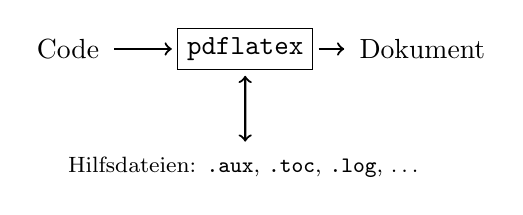
\begin{tikzpicture}[scale=.75,shorten <=2pt, shorten >=2pt]

            \node[rectangle]
            	(code) 		at (0,0) {Code};
            \node[rectangle,draw,fill=white]
            	(latex) 	at (3,0) {\texttt{pdflatex}};
            \node[rectangle]
            	(dokument) 	at (6,0) {Dokument};
            \node
            	(aux) at (3,-2) {\footnotesize Hilfsdateien: \texttt{.aux}, \texttt{.toc},
            	\texttt{.log}, \ldots};
            \begin{scope}[thick]
                \path[->] (code)  edge (latex);
                \path[->] (latex) edge (dokument);
                \path[<->] (latex) edge (aux);
            \end{scope}
        \end{tikzpicture}
    \end{block}
\end{frame}
